% -------------------------------------------- %
%	Apêndices (configurar em arquivo externo)
% -------------------------------------------- %
% Etapas:
% 1. Criar um arquivo ".tex" na pasta "\material-de-apoio\apendices".
% 2. Configurar arquivo da etapa 1.
% 3. Neste arquivo ("apendices.tex") copiar estrutura do "Apêndice A".

% Apêndice A ..................................................
\begin{appendices}
\chapter{}
% ------------------------------------------- %
%	Apêndice A (alterar conforme necessidade)
% ------------------------------------------- %

De acordo com a NBR 14724:2011 é um elemento opcional. É o texto ou documento elaborado pelo autor, a fim de complementar sua argumentação. Deve ser apresentado em folha própria com numeração contínua à do texto principal, na qual deve ser colocado a palavra Apêndice em letra maiúscula e a letra de identificação, seguidos de travessão e em letra minúscula o título do apêndice.
\clearpage
\newpage
\end{appendices}
\newpage

% Apêndice B ..................................................
\begin{appendices}
\chapter{}
% ------------------------------------------- %
%	Apêndice B (alterar conforme necessidade)
% ------------------------------------------- %
% Inserir a primeira página do pdf (procedimento necessário para não ficar com página em branco)
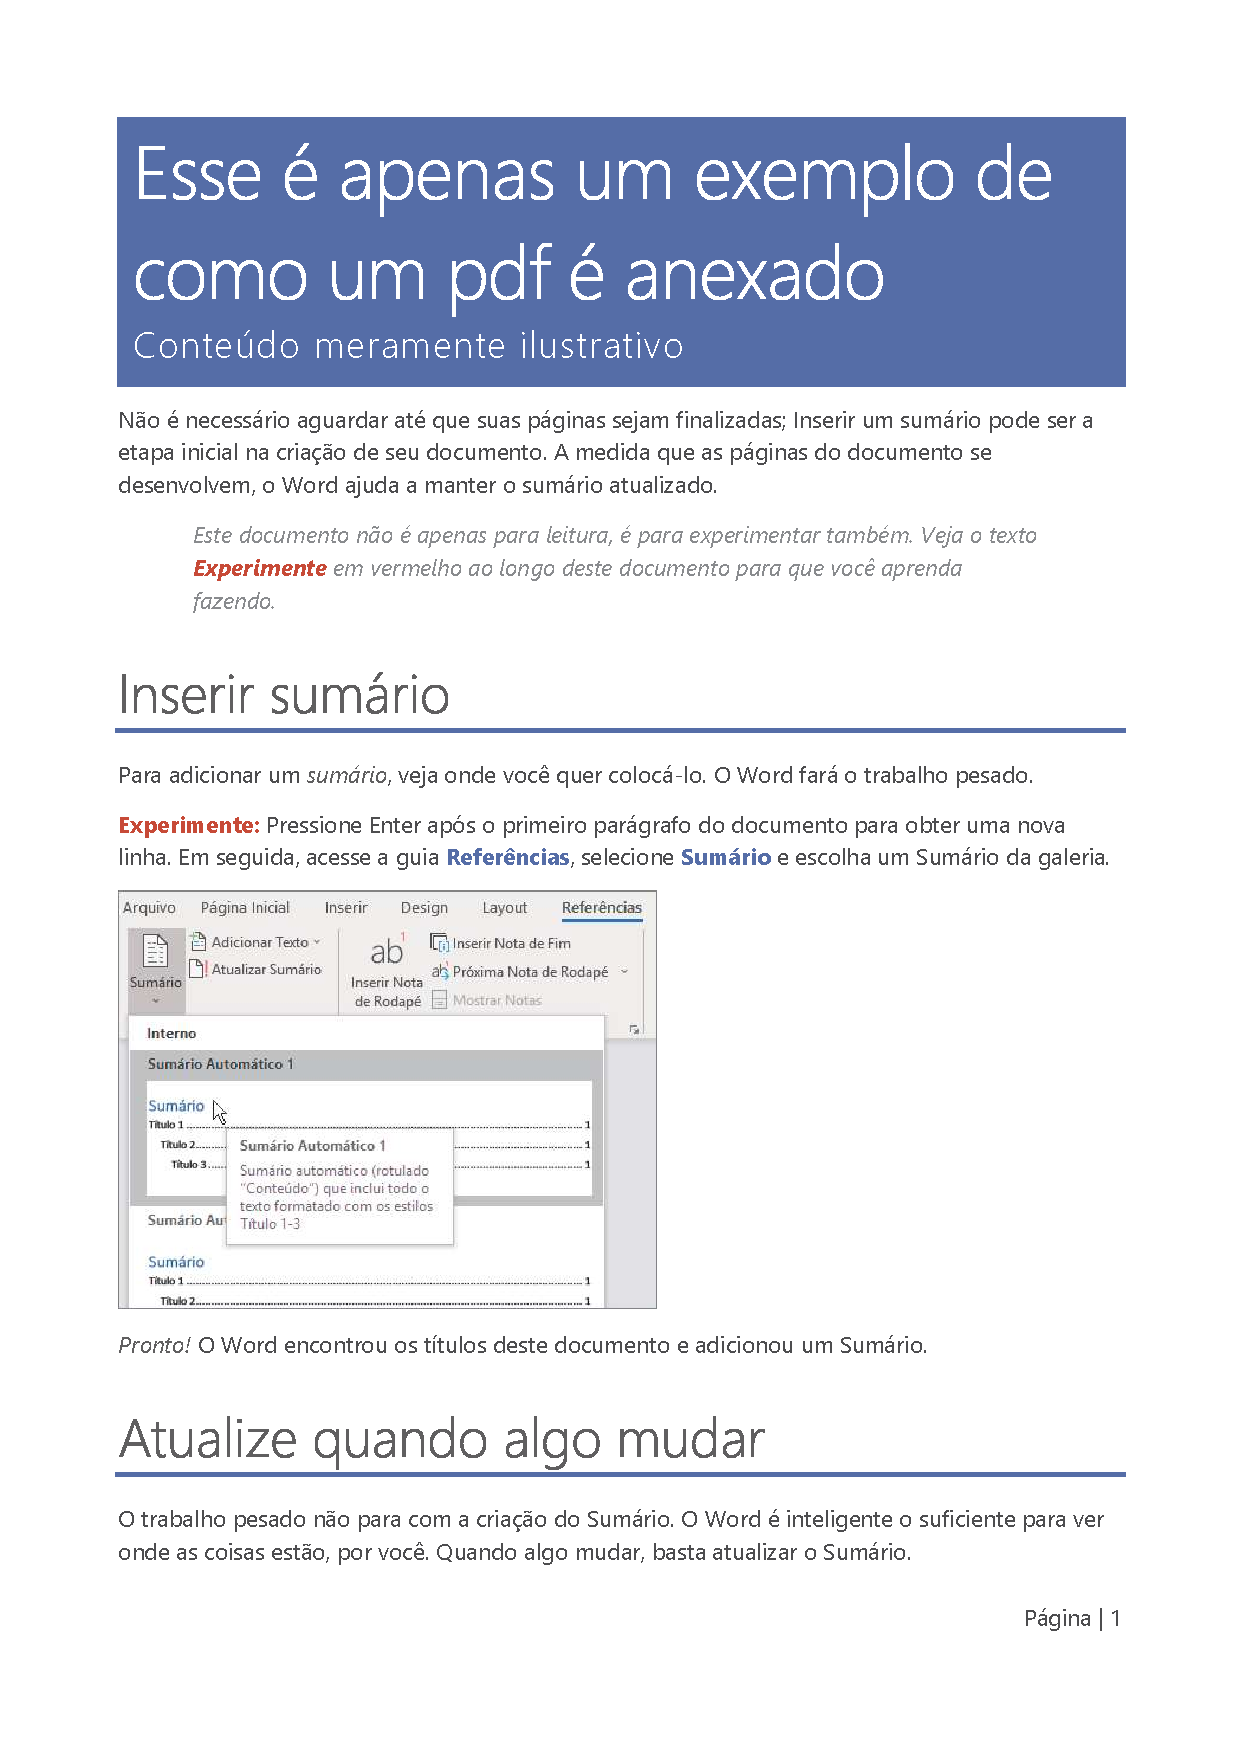
\includegraphics[page=1,width=0.9\linewidth,height=0.9\textheight]{material-de-apoio/pdfs/storopoli-et-al_2021_Simulation-Driven_COVID-19.pdf}

% Inserir demais páginas do pdf
\includepdf[pages={2-},scale=0.80,pagecommand={}]{material-de-apoio/pdfs/storopoli-et-al_2021_Simulation-Driven_COVID-19.pdf}

\newpage
\end{appendices}
\newpage